% =====================================================================
%  V2V-Project -- Study Pack
%  Section S1 : The Big Picture and Threat Model
%  Source files studied: readme.md , config.py
%  Standalone document -- compile with:  pdflatex 01-big-picture-threat-model.tex
% =====================================================================
\documentclass[11pt,a4paper]{article}

% ---- encoding & fonts ----
\usepackage[utf8]{inputenc}
\usepackage[T1]{fontenc}
\usepackage{lmodern}

% ---- layout ----
\usepackage[a4paper,margin=2.4cm]{geometry}
\usepackage{enumitem}
\setlist{topsep=2pt,itemsep=2pt}

% ---- maths, tables, graphics ----
\usepackage{amsmath}
\usepackage{amssymb}
\usepackage{booktabs}
\usepackage{graphicx}
\usepackage{xcolor}

% ---- code listings ----
\usepackage{listings}

% ---- diagrams ----
\usepackage{tikz}
\usetikzlibrary{arrows.meta,positioning,shapes.geometric,calc,fit,backgrounds}

% ---- hyperlinks (load late) ----
\usepackage[colorlinks=true,linkcolor=blue,urlcolor=blue,citecolor=blue]{hyperref}

% ---------------------------------------------------------------------
%  Colours and code style
% ---------------------------------------------------------------------
\definecolor{codebg}{rgb}{0.97,0.97,0.94}
\definecolor{codegreen}{rgb}{0.00,0.50,0.00}
\definecolor{codegray}{rgb}{0.50,0.50,0.50}
\definecolor{keyblue}{rgb}{0.00,0.20,0.70}
\definecolor{boxblue}{rgb}{0.88,0.93,1.00}
\definecolor{boxyellow}{rgb}{1.00,0.97,0.85}

\lstdefinestyle{py}{
  language=Python,
  backgroundcolor=\color{codebg},
  basicstyle=\ttfamily\footnotesize,
  keywordstyle=\color{keyblue}\bfseries,
  stringstyle=\color{codegreen},
  commentstyle=\color{codegray}\itshape,
  numberstyle=\tiny\color{codegray},
  numbers=left,
  numbersep=8pt,
  showstringspaces=false,
  breaklines=true,
  breakatwhitespace=false,
  frame=single,
  rulecolor=\color{codegray},
  tabsize=4,
  captionpos=b,
}
\lstdefinestyle{term}{
  backgroundcolor=\color{codebg},
  basicstyle=\ttfamily\footnotesize,
  breaklines=true,
  frame=single,
  rulecolor=\color{codegray},
  numbers=none,
  captionpos=b,
}

% ---------------------------------------------------------------------
\title{\textbf{V2V-Project Study Pack}\\[4pt]
       \large Section S1 --- The Big Picture and Threat Model}
\author{Information Security Project --- Beginner Study Notes}
\date{Source files: \texttt{readme.md}, \texttt{config.py}}

\begin{document}
\maketitle
\tableofcontents
\newpage

% =====================================================================
\section{Title and ``What You'll Learn''}
% =====================================================================

\subsection*{Section Title}
\textbf{S1 --- The Big Picture and Threat Model of the V2V Communication
Security Simulation.}

\subsection*{Plain-English Summary (read this first)}
This project is a small computer program, written in Python, that pretends to
be two cars talking to each other on a road. The cars send tiny ``I am here,
this is my speed'' safety messages. The catch is that the radio link between
them is \emph{untrusted} --- a stranger could listen in, change the words, or
pretend to be one of the cars. Section~S1 does not teach a single piece of code
in depth; instead it gives you the \emph{map of the whole project}: what problem
it solves, who the attacker is, what the four attacks are, and what six
``security properties'' the project promises to deliver. Once you understand
S1, every later section (the certificates, the encryption maths, the handshake)
will have a place to fit.

\subsection*{Learning Outcomes}
After studying this section you will be able to:
\begin{itemize}
  \item Explain in one sentence what ``Vehicle-to-Vehicle (V2V) communication''
        is and why it needs protecting.
  \item Define a \textbf{Basic Safety Message (BSM)} and say how often it is sent.
  \item Describe the \textbf{threat model}: who the attacker is and what powers
        they have over the network.
  \item Name and describe the \textbf{four attacks} the project defends against:
        replay, tamper, man-in-the-middle (MITM), and impersonation.
  \item Name and explain the \textbf{six security properties}: confidentiality,
        integrity, authentication, non-repudiation, forward secrecy, and
        replay prevention.
  \item Describe the three-stage pipeline --- Identity, Authentication, Secure
        Messaging --- and which project files belong to each stage.
  \item Read \texttt{config.py} and explain what every shared constant controls.
\end{itemize}

% =====================================================================
\section{Where This Fits}
% =====================================================================

S1 is the ``cover page'' of the whole system. Every other section is one
component; S1 is the picture on the jigsaw box that tells you what the finished
puzzle looks like. The project is built as a \textbf{pipeline of three stages},
and the readme describes them in exactly this order:

\begin{enumerate}
  \item \textbf{Identity} --- ``Who are you?'' Each vehicle is given a digital
        passport (a \emph{certificate}) by a trusted authority. Files:
        \texttt{ca/ca.py}, \texttt{ca/issue\_cert.py}, \texttt{ca/verify\_cert.py}
        (this is Section~S2).
  \item \textbf{Authentication} --- ``Prove it!'' Before talking, the two
        vehicles run a four-step handshake to check each other's passport and
        agree on a secret key. File: \texttt{protocol/auth\_protocol.py}
        (Section~S4), built on the crypto core
        \texttt{crypto/crypto.py} (Section~S3).
  \item \textbf{Secure Messaging} --- ``Sign, then encrypt.'' Now the vehicles
        exchange safety messages, each one stamped and sealed. File:
        \texttt{protocol/v2v\_protocol.py} (Section~S5).
\end{enumerate}

\noindent The remaining files support these stages: \texttt{node/vehicle\_node.py}
runs the networking, \texttt{dashboard/app.py} shows a live monitoring screen,
the \texttt{attacks/} scripts try to break the system, and
\texttt{tests/evaluate\_security.py} measures how well it holds up.
\textbf{\texttt{config.py}} is the small file of shared settings that every
stage reads from.

\begin{center}
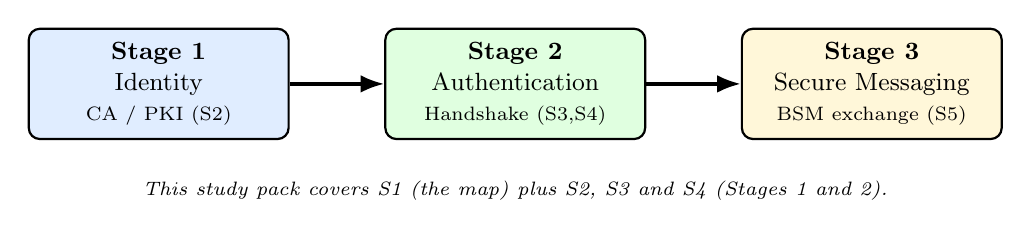
\begin{tikzpicture}[node distance=10mm and 12mm,
    every node/.style={font=\small},
    stage/.style={draw,rounded corners,minimum width=3.3cm,minimum height=1.4cm,
                  align=center,thick}]
  \node[stage,fill=boxblue]   (id)   {\textbf{Stage 1}\\Identity\\\scriptsize CA / PKI (S2)};
  \node[stage,fill=green!12,right=of id]   (auth) {\textbf{Stage 2}\\Authentication\\\scriptsize Handshake (S3,S4)};
  \node[stage,fill=boxyellow,right=of auth] (msg) {\textbf{Stage 3}\\Secure Messaging\\\scriptsize BSM exchange (S5)};
  \draw[-{Latex[length=3mm]},very thick] (id)   -- (auth);
  \draw[-{Latex[length=3mm]},very thick] (auth) -- (msg);
  \node[below=4mm of auth,font=\scriptsize\itshape,align=center]
       {This study pack covers S1 (the map) plus S2, S3 and S4 (Stages 1 and 2).};
\end{tikzpicture}
\end{center}

% =====================================================================
\section{The Theory You Must Study}
% =====================================================================

\subsection{Vehicle-to-Vehicle (V2V) Communication}
\textbf{Plain definition.} V2V communication means cars wirelessly broadcasting
short messages to nearby cars about their position, speed and movement, so the
cars (or their drivers) can react to danger faster than a human could.

\textbf{Real-life analogy.} Imagine every car has a loudspeaker on its roof
constantly calling out ``I am here, going 80, turning left''. Other cars hear
this and brake or steer in time.

\textbf{Why it exists / what problem it solves.} Human reaction time is slow and
a driver cannot see around a blind corner or through the truck in front. V2V
lets a car ``see'' a sudden brake three vehicles ahead and react in
milliseconds, preventing pile-ups.

\textbf{How it works at a beginner level.} Each car has a small radio. Several
times every second it sends a tiny message. Nearby cars receive it and update
their picture of the traffic around them. \emph{In this project the radio is
simulated by an ordinary TCP network connection between two programs.}

\textbf{Security property it relates to.} None on its own --- V2V is just the
\emph{communication}. The danger is precisely that, by default, this
communication has \emph{no} security at all. Everything else in the project
exists to add security on top.

\subsection{Basic Safety Message (BSM)}
\textbf{Plain definition.} A BSM is the small data packet a vehicle broadcasts.
It contains facts such as speed, heading (which way the car points), location,
and whether the brakes are on.

\textbf{Real-life analogy.} A BSM is like a quick status shout: ``Speed 80,
heading 45 degrees, not braking.'' It is short, said often, and instantly
forgotten once newer information arrives.

\textbf{Why it exists.} Cars need a \emph{standard, tiny} message so the radio
channel is not flooded and every car understands every other car. Real systems
(the SAE~J2735 standard) broadcast a BSM about ten times per second.

\textbf{How it works here.} In this project the readme states a BSM is sent
\emph{once per second} --- controlled by the constant
\texttt{BSM\_SEND\_INTERVAL = 1.0} in \texttt{config.py}. A BSM carries fields
like speed, heading and a braking flag. (Real V2V sends BSMs about ten times a
second; the project slows this to once a second so a human watching the
dashboard can follow along. This is a deliberate simplification.)

\textbf{Security property it relates to.} A BSM is the \emph{thing being
protected}. All six security properties below are promises about what happens
to a BSM as it crosses the network.

\subsection{The Untrusted Channel and the Threat Model}
\textbf{Plain definition.} A \emph{threat model} is a clear written statement of
\emph{who might attack you} and \emph{what they are able to do}. An
\emph{untrusted channel} is a communication link you must assume the enemy
controls.

\textbf{Real-life analogy.} Posting a letter through a postal service run by
nosy, dishonest staff: they can read your letter, rewrite it, throw it away,
copy it and post the copy again next week, or even write a brand-new letter and
sign your name.

\textbf{Why it exists.} You cannot defend against an attacker you have not
described. The threat model forces the designer to be honest: ``assume the worst
about the network.''

\textbf{How it works here.} The readme's threat model assumes an attacker who
fully controls the channel between Vehicle~A and Vehicle~B. That attacker can:
\begin{itemize}
  \item \textbf{Eavesdrop} --- read every message that passes.
  \item \textbf{Tamper} --- change the contents of a message in transit.
  \item \textbf{Impersonate} --- pretend to be a legitimate vehicle.
  \item \textbf{Replay} --- record a real message and send it again later.
\end{itemize}
The project does \emph{not} try to defend against an attacker who has stolen a
vehicle's secret private key files from its hard disk, or against denial of
service (jamming the radio so no message gets through). Those are out of scope
--- a normal and honest limitation for a student project.

\textbf{Security property it relates to.} The threat model is the question;
the six security properties are the answer.

\subsection{The Four Attacks}

\subsubsection*{(a) Replay Attack}
\textbf{Definition.} The attacker copies a genuine, valid message and re-sends
the exact same bytes later.

\textbf{Analogy.} Recording someone saying ``open the door'' and playing the
recording back tomorrow to get in.

\textbf{The danger.} Re-sending an old ``I am braking hard!'' message could make
cars behind brake for no reason and cause a crash.

\textbf{Project defence.} Every message carries a \emph{timestamp}; messages
older than \texttt{TIMESTAMP\_MAX\_AGE = 5.0} seconds are rejected. Every message
also carries a one-time random number (a \emph{nonce}); once a nonce has been
seen it is remembered for \texttt{REPLAY\_WINDOW\_SECONDS = 300} seconds and any
repeat is rejected. Demo script: \texttt{attacks/replay\_attack.py}.

\subsubsection*{(b) Tamper Attack}
\textbf{Definition.} The attacker intercepts a message and changes part of it,
e.g. flips ``speed: 60'' to ``speed: 0''.

\textbf{Analogy.} Steaming open a sealed envelope, editing the letter inside,
and re-sealing it --- except here the seal is mathematical and cannot be faked.

\textbf{The danger.} False speed or position data makes other cars make wrong,
dangerous decisions.

\textbf{Project defence.} The encryption used, AES-256-GCM, produces a 128-bit
\emph{authentication tag} computed over the whole ciphertext. Changing even one
bit makes the tag mismatch and decryption fails immediately. Demo:
\texttt{attacks/tamper\_attack.py}.

\subsubsection*{(c) Man-in-the-Middle (MITM) Attack}
\textbf{Definition.} The attacker secretly sits between A and B, relaying (and
possibly altering) every message, while each side believes it is talking
directly to the other.

\textbf{Analogy.} A dishonest interpreter standing between two people who do not
share a language: each trusts the interpreter completely, so the interpreter can
quietly change every sentence.

\textbf{The danger.} The attacker could read or rewrite the entire conversation.

\textbf{Project defence.} Two layers. (Scenario~A) If the attacker offers a
\emph{fake certificate}, it is rejected because it is not signed by the trusted
CA. (Scenario~B) If the attacker tries to \emph{forge a signature}, it fails
because they do not own the vehicle's private key. Demo:
\texttt{attacks/mitm\_attack.py}.

\subsubsection*{(d) Impersonation / Spoofing}
\textbf{Definition.} The attacker pretends to be Vehicle~A without being
Vehicle~A.

\textbf{Analogy.} A stranger walking up to a border using a passport with
someone else's name on it.

\textbf{The danger.} A fake car could inject false safety messages and direct
real cars into danger.

\textbf{Project defence.} Each real vehicle has a certificate signed by the CA
\emph{and} a private key that only it owns. During the handshake a vehicle must
sign a fresh random challenge; only the true owner of the private key can
produce a signature that verifies. Impersonation overlaps with MITM Scenario~B
and is handled by the same handshake (Section~S4).

\subsection{The Six Security Properties}
A ``security property'' is a promise the system keeps. Table~\ref{tab:props}
lists the six the project claims, exactly as written in the readme.

\begin{table}[h]
\centering
\small
\begin{tabular}{@{}p{2.9cm} p{5.0cm} p{5.6cm}@{}}
\toprule
\textbf{Property} & \textbf{Plain meaning} & \textbf{How the project achieves it}\\
\midrule
Confidentiality & Only the intended car can read the message. &
AES-256-GCM encryption with a shared session key.\\
Integrity & The message cannot be changed without it being noticed. &
The 128-bit AES-GCM authentication tag.\\
Authentication & Each car proves who it really is. &
X.509 certificates plus the 4-step handshake.\\
Non-repudiation & A sender cannot later deny it sent the message. &
An ECDSA digital signature on every BSM.\\
Forward secrecy & Stealing a key tomorrow does not unlock today's messages. &
Fresh (ephemeral) ECDH keys generated per session.\\
Replay prevention & An old message cannot be reused. &
Nonce cache plus a 5-second timestamp window.\\
\bottomrule
\end{tabular}
\caption{The six security properties promised by the V2V project.}
\label{tab:props}
\end{table}

\textbf{One honest clarification about ``5 seconds''.} The readme's property
table summarises replay prevention as a ``5s window'', but the code actually
uses \emph{two} separate windows, and it helps to keep them apart:
\begin{itemize}
  \item \texttt{TIMESTAMP\_MAX\_AGE = 5.0} --- a message whose timestamp is more
        than 5~seconds away from ``now'' is rejected as \emph{stale}.
  \item \texttt{REPLAY\_WINDOW\_SECONDS = 300} --- each nonce that has been seen
        is \emph{remembered} for 300~seconds (5~minutes), so an exact repeat
        within that window is caught even if its timestamp were somehow fresh.
\end{itemize}
Together they form a belt-and-braces defence: the timestamp catches \emph{old}
messages cheaply, and the nonce cache catches \emph{exact duplicates}.

% =====================================================================
\section{Code Walkthrough}
% =====================================================================

Section~S1 has no large algorithm to trace. Its ``code'' is the project's
shared settings file, \texttt{config.py}. Every other module imports its numbers
from here so that there is a single, easy-to-find place to change behaviour.
Below is the real file, followed by a step-by-step explanation of every group.

\begin{lstlisting}[style=py,caption={config.py --- shared constants for the
whole simulation (decorative dashes in the original comments shortened to
plain ASCII for printing).}]
"""Shared configuration constants for the V2V security simulation."""

# -- Network Configuration --
VEHICLE_A_PORT = 9001          # TCP port Vehicle A listens on
VEHICLE_B_PORT = 9002          # TCP port Vehicle B listens on
DASHBOARD_A_PORT = 5001        # Flask dashboard for Vehicle A
DASHBOARD_B_PORT = 5002        # Flask dashboard for Vehicle B

# -- Certificate Paths --
CA_CERT_PATH = "ca/certs/ca_cert.pem"
CA_KEY_PATH = "ca/certs/ca_key.pem"
VEHICLE_A_CERT = "ca/certs/vehicle-a_cert.pem"
VEHICLE_A_KEY = "ca/certs/vehicle-a_key.pem"
VEHICLE_B_CERT = "ca/certs/vehicle-b_cert.pem"
VEHICLE_B_KEY = "ca/certs/vehicle-b_key.pem"

# -- Security Parameters --
REPLAY_WINDOW_SECONDS = 300    # Nonces remembered for 5 minutes
TIMESTAMP_MAX_AGE = 5.0        # Messages older than 5 seconds are rejected
BSM_SEND_INTERVAL = 1.0        # Send a BSM every 1 second

# -- Crypto Settings --
AES_KEY_LENGTH = 32            # 256 bits (AES-256)
NONCE_LENGTH = 12              # 96 bits (AES-GCM standard nonce size)
EC_CURVE = "secp256r1"         # NIST P-256 curve (same as TLS 1.3)
SESSION_KEY_INFO = b"v2v-session-key-v1"  # HKDF info string

# -- Simulation Settings --
SIMULATED_LATITUDE = 6.9271    # Colombo, Sri Lanka
SIMULATED_LONGITUDE = 79.8612
SPEED_RANGE = (60.0, 100.0)    # km/h for simulated vehicle
\end{lstlisting}

\subsection{Group 1 --- Network Configuration}
\textbf{Purpose:} tells each program which ``door numbers'' (TCP ports) to use.
\begin{enumerate}
  \item A \emph{port} is a numbered door on a computer; a program listens behind
        one door so messages can find it.
  \item \texttt{VEHICLE\_A\_PORT = 9001} and \texttt{VEHICLE\_B\_PORT = 9002}:
        the two cars listen on ports 9001 and 9002.
  \item \texttt{DASHBOARD\_A\_PORT = 5001} and \texttt{DASHBOARD\_B\_PORT = 5002}:
        each car also runs a small web page (the dashboard) on its own port so
        you can watch it in a browser.
\end{enumerate}
\emph{Analogy:} ports are flat numbers in an apartment block --- the building
(computer) has one street address (IP), but the postman needs the flat number
to deliver to the right resident.

\subsection{Group 2 --- Certificate Paths}
\textbf{Purpose:} the file locations of every digital passport and key.
\begin{enumerate}
  \item \texttt{CA\_CERT\_PATH} / \texttt{CA\_KEY\_PATH}: the trusted authority's
        public certificate and its secret signing key.
  \item \texttt{VEHICLE\_A\_CERT} / \texttt{VEHICLE\_A\_KEY} (and the B pair):
        each vehicle's own passport and matching private key.
  \item All files end in \texttt{.pem}. PEM (Privacy-Enhanced Mail) is just a
        text format for storing keys and certificates --- you will meet it in
        detail in Section~S2.
\end{enumerate}
\emph{Tie to theory:} this group is the ``Identity'' stage on paper --- it
records where the passports live.

\subsection{Group 3 --- Security Parameters}
\textbf{Purpose:} the timing rules that stop replay attacks.
\begin{enumerate}
  \item \texttt{REPLAY\_WINDOW\_SECONDS = 300}: how long a used nonce is
        remembered. Implements the \emph{nonce cache} part of replay prevention.
  \item \texttt{TIMESTAMP\_MAX\_AGE = 5.0}: how stale a message may be before it
        is thrown away. Implements the \emph{freshness} part of replay
        prevention.
  \item \texttt{BSM\_SEND\_INTERVAL = 1.0}: send one safety message per second.
\end{enumerate}
\emph{Tie to theory:} this group is the numeric heart of the
\textbf{replay prevention} property.

\subsection{Group 4 --- Crypto Settings}
\textbf{Purpose:} the sizes and names of the cryptographic building blocks.
\begin{enumerate}
  \item \texttt{AES\_KEY\_LENGTH = 32}: the secret key is 32 bytes = 256 bits,
        hence ``AES-256''. Implements \textbf{confidentiality}.
  \item \texttt{NONCE\_LENGTH = 12}: the AES-GCM nonce is 12 bytes = 96 bits,
        the size recommended by the standard. (Note: this is the encryption
        nonce. The handshake in S4 uses a separate, larger 32-byte nonce ---
        do not confuse the two.)
  \item \texttt{EC\_CURVE = "secp256r1"}: the name of the elliptic curve used
        for keys --- the same NIST P-256 curve used by TLS~1.3 (the protocol
        behind HTTPS).
  \item \texttt{SESSION\_KEY\_INFO = b"v2v-session-key-v1"}: a label fed into the
        key-derivation step (HKDF) so the derived key is tied to this exact
        purpose.
\end{enumerate}
\emph{Honest note on accuracy:} \texttt{config.py} is meant to be the single
source of truth, but a few modules hard-code the same values directly instead of
importing them --- for example \texttt{crypto/crypto.py} writes
\texttt{os.urandom(12)} and the literal string \texttt{b"v2v-session-key-v1"}
itself rather than reading \texttt{NONCE\_LENGTH} and \texttt{SESSION\_KEY\_INFO}.
The numbers agree, so behaviour is correct, but it is good practice to notice
this duplication and mention it if an examiner asks ``is config.py actually
used everywhere?''

\subsection{Group 5 --- Simulation Settings}
\textbf{Purpose:} fake but realistic data so the cars have something to ``say''.
\begin{enumerate}
  \item \texttt{SIMULATED\_LATITUDE} / \texttt{SIMULATED\_LONGITUDE}: a fixed GPS
        location (Colombo, Sri Lanka) used as the starting point.
  \item \texttt{SPEED\_RANGE = (60.0, 100.0)}: the simulated car picks a speed
        between 60 and 100 km/h.
\end{enumerate}
\emph{Tie to theory:} this is the \emph{content of a BSM} --- the very data the
six security properties are protecting.

\medskip
\noindent\textbf{Why a config file at all?} If the port number or the timeout
were scattered across ten files, changing one would mean ten risky edits.
Centralising them is the same idea as a fuse box: all the switches in one labelled
panel. There are no function arguments, return values, or exceptions in
\texttt{config.py} --- it is pure data, executed once when imported.

% =====================================================================
\section{Hands-On / Practical}
% =====================================================================

S1 is the ``map'' section, so the practical work is to (1) confirm your tools
are installed, (2) inspect the shared settings, and (3) see the whole pipeline
run once end to end.

\subsection{Step 1 --- Check Python and the crypto library}
Open PowerShell in the project folder and run:
\begin{lstlisting}[style=term]
python --version
pip install cryptography flask requests pytest
\end{lstlisting}
You need Python 3.10 or newer. The \texttt{cryptography} library supplies all
the encryption maths used by S3 and S4.

\subsection{Step 2 --- Inspect the shared constants}
Run a one-line Python command that imports \texttt{config.py} and prints a few
values:
\begin{lstlisting}[style=term]
python -c "import config; print(config.AES_KEY_LENGTH, config.TIMESTAMP_MAX_AGE, config.BSM_SEND_INTERVAL)"
\end{lstlisting}

\noindent\textbf{Expected output:}
\begin{lstlisting}[style=term]
32 5.0 1.0
\end{lstlisting}
\textbf{What each number means:} \texttt{32} is the AES key length in bytes (a
256-bit key); \texttt{5.0} is the maximum age in seconds before a message is
treated as stale; \texttt{1.0} is the gap in seconds between safety messages.

\subsection{Step 3 --- Watch the whole pipeline once}
You can see all three stages in a single run by generating the certificates and
running the handshake demo (these belong to S2--S4 but together they show the
S1 big picture):
\begin{lstlisting}[style=term]
python ca\ca.py
python ca\issue_cert.py --vehicle-id vehicle-a --output-dir ca\certs
python ca\issue_cert.py --vehicle-id vehicle-b --output-dir ca\certs
python protocol\auth_protocol.py
\end{lstlisting}
The first three commands build Stage~1 (Identity); the last command runs
Stage~2 (Authentication) and ends by printing that both cars derived the
\emph{same} session key.

\subsection{Try This Yourself (mini-experiment)}
Open \texttt{config.py} and change one line:
\begin{lstlisting}[style=term]
TIMESTAMP_MAX_AGE = 5.0      ->   TIMESTAMP_MAX_AGE = 0.001
\end{lstlisting}
\textbf{Predict before you run.} 0.001~seconds is one millisecond. A message
almost always takes longer than a millisecond to build and travel, so by the
time it is checked it is already ``too old''. Prediction: the handshake or BSM
exchange should now \emph{fail} with a ``stale message'' error, even though
nothing malicious happened. This shows that security parameters are a balance ---
too strict and the honest system breaks; too loose and attacks slip through.
\textbf{Remember to change the value back to 5.0 afterwards.}

% =====================================================================
\section{Attack Relevance}
% =====================================================================

S1 does not itself contain a defence --- it is the chapter that \emph{names} the
attacks and the defences so the rest of the project has a target. Still, it is
directly relevant to all four attacks because it defines them and points to the
file that demonstrates each one.

\begin{table}[h]
\centering
\small
\begin{tabular}{@{}p{2.6cm} p{5.6cm} p{5.3cm}@{}}
\toprule
\textbf{Attack} & \textbf{What the attacker does} & \textbf{Which property/section stops it}\\
\midrule
Replay & Re-sends a captured valid message. &
Replay prevention --- timestamp + nonce cache (S4).\\
Tamper & Edits a message in transit. &
Integrity --- AES-GCM authentication tag (S3, S5).\\
MITM & Relays/alters traffic from the middle. &
Authentication --- certificates + handshake (S2, S4).\\
Impersonation & Pretends to be a real vehicle. &
Authentication + non-repudiation --- signed challenge (S2, S4).\\
\bottomrule
\end{tabular}
\caption{S1 maps each attack to the property and section that defeats it.}
\end{table}

\noindent The \texttt{config.py} constants \texttt{TIMESTAMP\_MAX\_AGE} and
\texttt{REPLAY\_WINDOW\_SECONDS} are the only S1 items that play a \emph{direct}
defensive role: they are the dials that tune how aggressively replay attacks are
rejected.

% =====================================================================
\section{Illustrations}
% =====================================================================

\subsection{Diagram 1 --- The Threat Model}
The attacker owns the channel. Figure below shows the honest vehicles at the
edges and the attacker controlling everything in between.

\begin{center}
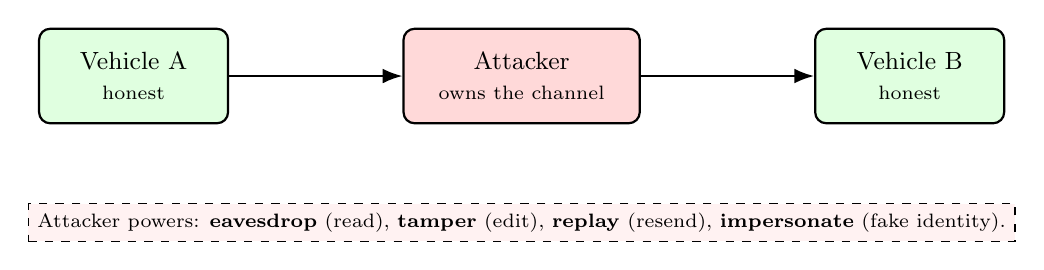
\begin{tikzpicture}[node distance=8mm,font=\small,
   car/.style={draw,thick,rounded corners,fill=green!12,minimum width=2.4cm,
               minimum height=1.2cm,align=center},
   atk/.style={draw,thick,rounded corners,fill=red!15,minimum width=3.0cm,
               minimum height=1.2cm,align=center}]
  \node[car] (a) {Vehicle A\\\scriptsize honest};
  \node[atk,right=22mm of a] (m) {Attacker\\\scriptsize owns the channel};
  \node[car,right=22mm of m] (b) {Vehicle B\\\scriptsize honest};
  \draw[-{Latex[length=2.5mm]},thick] (a) -- (m);
  \draw[-{Latex[length=2.5mm]},thick] (m) -- (b);
  \node[below=10mm of m,align=center,font=\scriptsize,draw,dashed,fill=red!5,
        minimum width=8.5cm]
       {Attacker powers: \textbf{eavesdrop} (read), \textbf{tamper} (edit),
        \textbf{replay} (resend), \textbf{impersonate} (fake identity).};
\end{tikzpicture}
\end{center}

\subsection{Diagram 2 --- The Three-Stage Pipeline with Files}
\begin{center}
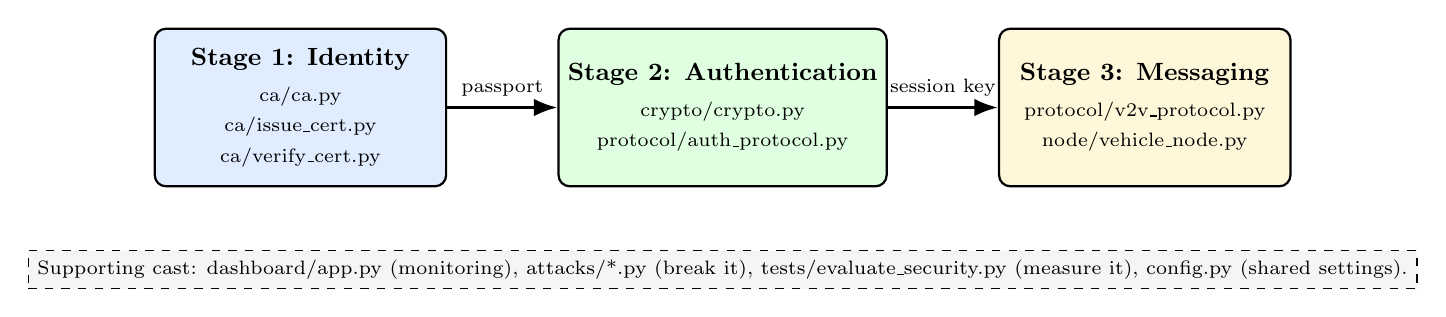
\begin{tikzpicture}[font=\small,node distance=6mm,
   box/.style={draw,rounded corners,minimum width=3.7cm,minimum height=2.0cm,
               align=center,thick}]
  \node[box,fill=boxblue]   (s1) {\textbf{Stage 1: Identity}\\[2pt]
        \scriptsize ca/ca.py\\\scriptsize ca/issue\_cert.py\\\scriptsize ca/verify\_cert.py};
  \node[box,fill=green!12,right=14mm of s1] (s2)
       {\textbf{Stage 2: Authentication}\\[2pt]
        \scriptsize crypto/crypto.py\\\scriptsize protocol/auth\_protocol.py};
  \node[box,fill=boxyellow,right=14mm of s2] (s3)
       {\textbf{Stage 3: Messaging}\\[2pt]
        \scriptsize protocol/v2v\_protocol.py\\\scriptsize node/vehicle\_node.py};
  \draw[-{Latex[length=3mm]},very thick] (s1) -- (s2)
       node[midway,above,font=\scriptsize]{passport};
  \draw[-{Latex[length=3mm]},very thick] (s2) -- (s3)
       node[midway,above,font=\scriptsize]{session key};
  \node[below=8mm of s2,draw,dashed,fill=gray!8,minimum width=11cm,
        align=center,font=\scriptsize]
       {Supporting cast: dashboard/app.py (monitoring), attacks/*.py (break it),
        tests/evaluate\_security.py (measure it), config.py (shared settings).};
\end{tikzpicture}
\end{center}

% =====================================================================
\section{Presentation Pack}
% =====================================================================

\subsection{Slide Outline}

\textbf{Slide 1 --- The Problem.}
\begin{itemize}
  \item Cars send tiny ``safety messages'' (BSMs) many times a second.
  \item The radio channel is untrusted --- anyone nearby can listen.
  \item No security by default: a stranger can read, change, copy or fake messages.
  \item One false ``I am braking'' message could cause a crash.
\end{itemize}

\textbf{Slide 2 --- The Threat Model (who is the enemy?).}
\begin{itemize}
  \item We assume the attacker fully controls the channel.
  \item Four powers: eavesdrop, tamper, replay, impersonate.
  \item Out of scope: stealing key files from a car, jamming the radio.
  \item ``Design for the worst attacker you can describe.''
\end{itemize}

\textbf{Slide 3 --- The Four Attacks.}
\begin{itemize}
  \item Replay --- resend an old valid message.
  \item Tamper --- edit a message in transit.
  \item MITM --- secretly relay/alter the whole conversation.
  \item Impersonation --- pretend to be a real vehicle.
  \item Each has a demo script in the \texttt{attacks/} folder.
\end{itemize}

\textbf{Slide 4 --- The Six Security Properties.}
\begin{itemize}
  \item Confidentiality, Integrity, Authentication.
  \item Non-repudiation, Forward secrecy, Replay prevention.
  \item Each property is a \emph{promise} kept by a specific technique.
  \item Show Table~\ref{tab:props} on screen.
\end{itemize}

\textbf{Slide 5 --- The Three-Stage Pipeline.}
\begin{itemize}
  \item Stage 1 Identity --- give every car a passport (CA).
  \item Stage 2 Authentication --- handshake to prove identity + share a key.
  \item Stage 3 Secure Messaging --- sign then encrypt every BSM.
  \item \texttt{config.py} is the shared settings file feeding all three.
\end{itemize}

\subsection{Speaker Talking Points (about 30--60 seconds each)}

\textbf{Slide 1.} ``Picture two cars on a highway. Modern cars can talk to each
other by radio, sending tiny status messages called Basic Safety Messages many
times a second --- speed, direction, braking. This is genuinely useful: a car
can warn the car behind it before a human even notices danger. But the radio
link is open air. Anyone with a receiver can join in. If we send these messages
with no protection, a stranger can read them, change them, or fake them --- and
a single false `I am braking hard' message could trigger a real crash. So the
project's job is to add a security layer.''

\textbf{Slide 2.} ``Before defending anything, a security engineer writes down
the threat model --- who the enemy is and what they can do. We make a deliberately
pessimistic assumption: the attacker completely owns the channel between the two
cars. They can listen to every message, change any message, copy a message and
send it again, or pretend to be one of the cars. We are honest about limits too:
we do not defend against someone physically stealing the secret key files from
inside a car, or jamming the radio entirely. Naming what you do not cover is part
of good security work.''

\textbf{Slide 3.} ``Those attacker powers turn into four concrete attacks. A
replay attack records a real message and plays it back later. A tamper attack
edits a message as it passes. A man-in-the-middle attack puts the attacker
secretly in the middle, like a dishonest interpreter relaying and changing every
sentence. And impersonation is simply pretending to be a car you are not. The
nice thing about this project is that each attack has its own script in the
attacks folder, so we can actually run the attack and watch it fail.''

\textbf{Slide 4.} ``For each attacker power we promise a security property.
Confidentiality means only the intended car can read the message. Integrity
means any change is detected. Authentication means each car proves who it is.
Non-repudiation means a sender cannot later deny what it sent. Forward secrecy
means that even if a key leaks tomorrow, today's messages stay secret. And replay
prevention means an old message cannot be reused. Six promises --- and every one
is kept by a specific, named technique we will see in later sections.''

\textbf{Slide 5.} ``Finally, the big picture. The system is a pipeline of three
stages. Stage one, Identity: a Certificate Authority gives every car a digital
passport. Stage two, Authentication: the two cars run a four-step handshake to
check passports and secretly agree on a shared key. Stage three, Secure
Messaging: every safety message is signed and then encrypted before it goes out.
One small file, config.py, holds the shared settings --- ports, timeouts, key
sizes --- so all three stages read the same numbers.''

\subsection{Live-Demo Script}
\begin{enumerate}
  \item \textbf{Show the settings.} Run
        \texttt{python -c "import config; print(config.TIMESTAMP\_MAX\_AGE)"}.
        Point at the \texttt{5.0} and say ``this is our replay-freshness dial.''
  \item \textbf{Show the project map.} Open the folder in the editor; point at
        the \texttt{ca/}, \texttt{crypto/}, \texttt{protocol/}, \texttt{attacks/}
        folders and link each to a stage.
  \item \textbf{Run the pipeline.} Execute the four commands from
        Hands-On Step~3. Point at the final line ``both vehicles share the same
        key'' --- that is the whole project working in miniature.
  \item \textbf{Optional break-it moment.} Edit \texttt{TIMESTAMP\_MAX\_AGE} to
        \texttt{0.001}, re-run the handshake, and point at the ``stale message''
        failure to show parameters matter. Restore it to \texttt{5.0}.
\end{enumerate}

\subsection{Examiner Q\&A}
\begin{enumerate}
  \item \textbf{Q: What is a BSM and how often is it sent here?}\\
        A: A Basic Safety Message --- a small packet with speed, heading,
        location and braking state. In this project it is sent once per second
        (\texttt{BSM\_SEND\_INTERVAL = 1.0}); real V2V sends about ten per
        second, slowed here so a human can follow the dashboard.
  \item \textbf{Q: What is a threat model and what is this project's?}\\
        A: A written statement of who attacks and what they can do. Here: an
        attacker who fully controls the channel and can eavesdrop, tamper,
        replay and impersonate. Out of scope: stolen key files and jamming.
  \item \textbf{Q: Name the four attacks and one defence for each.}\\
        A: Replay (timestamp + nonce cache), Tamper (AES-GCM auth tag), MITM
        (CA-signed certificates), Impersonation (signed challenge proving
        private-key ownership).
  \item \textbf{Q: Name the six security properties.}\\
        A: Confidentiality, integrity, authentication, non-repudiation, forward
        secrecy, replay prevention.
  \item \textbf{Q: Difference between confidentiality and integrity?}\\
        A: Confidentiality hides the content (attacker cannot \emph{read} it);
        integrity protects the content (attacker cannot \emph{change} it
        undetected). AES-256-GCM gives both at once.
  \item \textbf{Q: Why two replay windows --- 5 seconds and 300 seconds?}\\
        A: \texttt{TIMESTAMP\_MAX\_AGE} (5\,s) cheaply rejects old messages;
        \texttt{REPLAY\_WINDOW\_SECONDS} (300\,s) remembers each nonce so an
        exact duplicate is caught even within the freshness window. Two layers,
        belt and braces.
  \item \textbf{Q: What is the purpose of config.py?}\\
        A: A single, central place for shared constants (ports, timeouts, key
        sizes) so a setting is changed once, not in many files.
  \item \textbf{Q: Is this a complete, real V2V system?}\\
        A: No --- it is a faithful \emph{simulation}. Real V2V uses dedicated
        radio (DSRC/C-V2X) and broadcasts to many cars; this project uses TCP
        between two programs and slows the message rate. The cryptography,
        however, is the same industry-standard set used by TLS.
\end{enumerate}

% =====================================================================
\section{Glossary}
% =====================================================================
\begin{description}[style=nextline,leftmargin=0pt]
  \item[V2V] Vehicle-to-Vehicle: cars exchanging wireless messages directly.
  \item[BSM] Basic Safety Message: the small status packet a vehicle broadcasts.
  \item[Threat model] A written description of who might attack and what they can do.
  \item[Untrusted channel] A communication link assumed to be under attacker control.
  \item[Eavesdrop] To secretly read messages in transit.
  \item[Tamper] To change a message's contents in transit.
  \item[Replay attack] Re-sending a previously captured valid message.
  \item[MITM] Man-in-the-Middle: an attacker secretly relaying/altering traffic.
  \item[Impersonation] Pretending to be a legitimate party (spoofing identity).
  \item[Confidentiality] Property: only the intended recipient can read a message.
  \item[Integrity] Property: any change to a message is detected.
  \item[Authentication] Property: each party proves who it really is.
  \item[Non-repudiation] Property: a sender cannot later deny having sent a message.
  \item[Forward secrecy] Property: past messages stay secret even if a key leaks later.
  \item[Replay prevention] Property: an old message cannot be reused.
  \item[Nonce] ``Number used once'': a one-time random value that detects duplicates.
  \item[Timestamp] A recorded time, used here to reject stale messages.
  \item[CA] Certificate Authority: the trusted issuer of digital passports.
  \item[Certificate] A digital passport binding an identity to a public key.
  \item[PEM] A text file format for storing keys and certificates.
  \item[Port] A numbered ``door'' on a computer that a program listens behind.
  \item[TCP] Transmission Control Protocol: a reliable network connection type.
  \item[AES-256-GCM] The authenticated encryption algorithm used for confidentiality + integrity.
  \item[ECDSA] Elliptic Curve Digital Signature Algorithm: proves who wrote a message.
  \item[ECDH] Elliptic Curve Diffie-Hellman: lets two parties agree a shared secret.
  \item[HKDF] A function that turns a raw shared secret into a clean usable key.
  \item[Session key] A temporary secret key used to encrypt one conversation.
  \item[config.py] The project's shared-settings file.
\end{description}

% =====================================================================
\section{References and Further Study}
% =====================================================================
\begin{itemize}
  \item \textbf{V2V overview (NHTSA, US road-safety agency)} ---
        \url{https://www.nhtsa.gov/research-data/vehicle-vehicle-communication}\\
        Read for: why V2V exists and the real-world safety case.
  \item \textbf{Vehicular communication systems (Wikipedia)} ---
        \url{https://en.wikipedia.org/wiki/Vehicular_communication_systems}\\
        Read for: a plain-English overview of the whole field.
  \item \textbf{SAE J2735 message-set standard} ---
        \url{https://www.sae.org/standards/content/j2735_202309/}\\
        Read for: the real definition of the Basic Safety Message.
  \item \textbf{IEEE 1609.2 (security for V2X)} ---
        \url{https://standards.ieee.org/ieee/1609.2/10258/}\\
        Read for: how real V2V security and certificates work.
  \item \textbf{Information security / the CIA triad (Wikipedia)} ---
        \url{https://en.wikipedia.org/wiki/Information_security}\\
        Read for: confidentiality, integrity, availability explained.
  \item \textbf{Replay attack (Wikipedia)} ---
        \url{https://en.wikipedia.org/wiki/Replay_attack}\\
        Read for: how replay works and standard defences.
  \item \textbf{Man-in-the-middle attack (Wikipedia)} ---
        \url{https://en.wikipedia.org/wiki/Man-in-the-middle_attack}\\
        Read for: the MITM concept and why authentication stops it.
  \item \textbf{Non-repudiation (Wikipedia)} ---
        \url{https://en.wikipedia.org/wiki/Non-repudiation}\\
        Read for: why digital signatures give non-repudiation.
  \item \textbf{Forward secrecy (Wikipedia)} ---
        \url{https://en.wikipedia.org/wiki/Forward_secrecy}\\
        Read for: why ephemeral keys protect past sessions.
  \item \textbf{Threat modelling (OWASP)} ---
        \url{https://owasp.org/www-community/Threat_Modeling}\\
        Read for: how professionals build a threat model.
  \item \textbf{NIST Computer Security Resource Center glossary} ---
        \url{https://csrc.nist.gov/glossary}\\
        Read for: precise definitions of every security term.
  \item \textbf{Python cryptography library documentation} ---
        \url{https://cryptography.io/en/latest/}\\
        Read for: the library this whole project is built on (used heavily in S2--S5).
\end{itemize}

\vfill
\begin{center}\footnotesize\itshape
End of Section S1. Next: S2 --- Public Key Infrastructure / Certificate Authority.
\end{center}

\end{document}
